% Created by tikzDevice version 0.11 on 2018-04-09 15:27:55
% !TEX encoding = UTF-8 Unicode
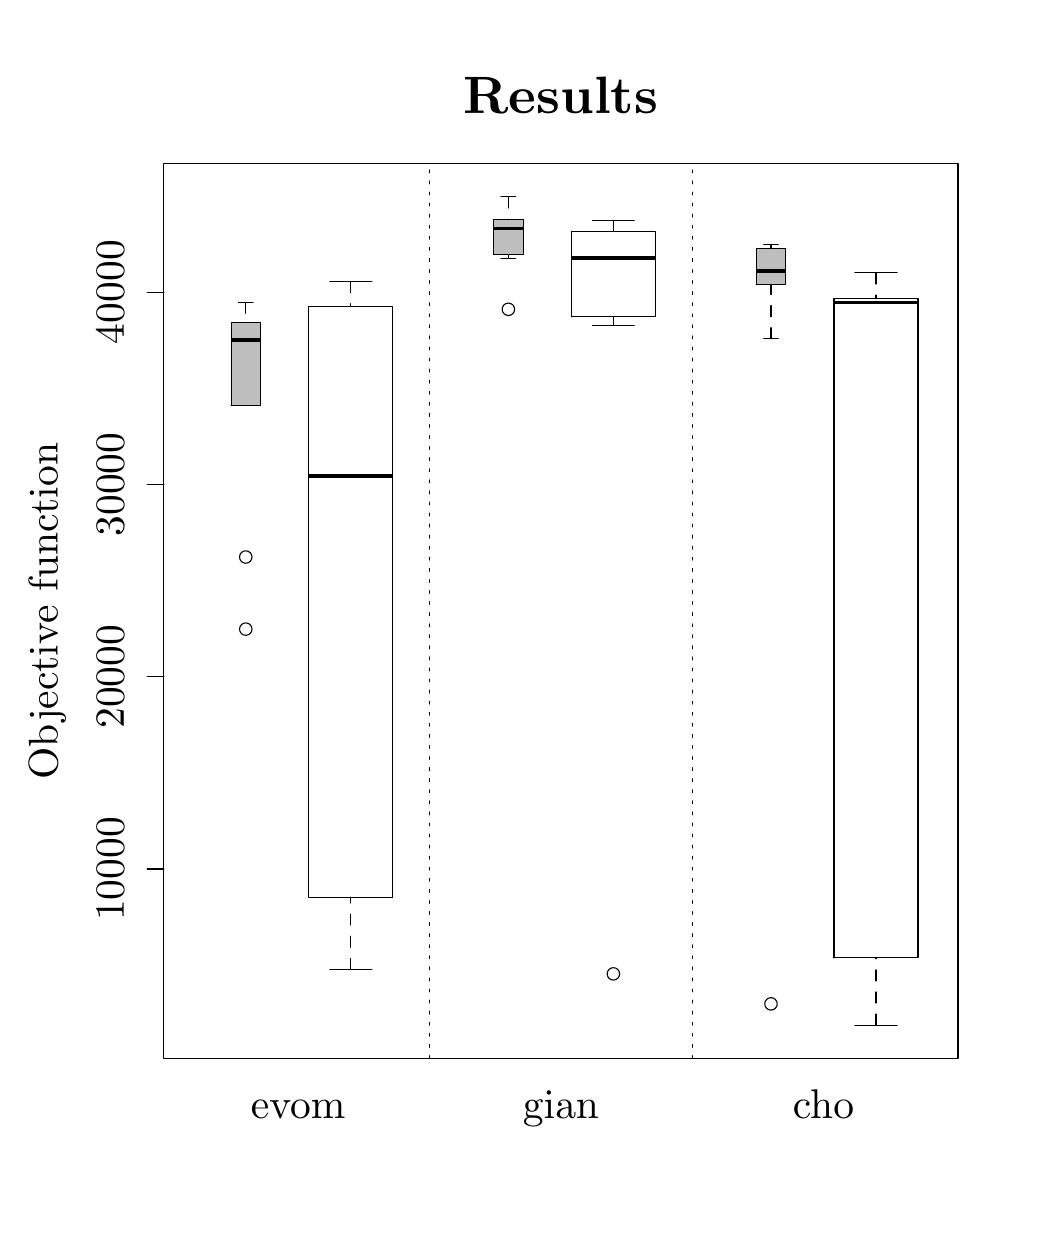
\begin{tikzpicture}[x=1pt,y=1pt]
\definecolor{fillColor}{RGB}{255,255,255}
\path[use as bounding box,fill=fillColor,fill opacity=0.00] (0,0) rectangle (361.35,433.62);
\begin{scope}
\path[clip] ( 49.20, 61.20) rectangle (336.15,384.42);
\definecolor{fillColor}{RGB}{190,190,190}

\path[fill=fillColor] ( 73.49,297.05) --
	( 84.12,297.05) --
	( 84.12,327.09) --
	( 73.49,327.09) --
	cycle;
\definecolor{drawColor}{RGB}{0,0,0}

\path[draw=drawColor,line width= 1.2pt,line join=round] ( 73.49,320.70) -- ( 84.12,320.70);

\path[draw=drawColor,line width= 0.4pt,dash pattern=on 4pt off 4pt ,line join=round,line cap=round] ( 78.81,297.05) -- ( 78.81,297.05);

\path[draw=drawColor,line width= 0.4pt,dash pattern=on 4pt off 4pt ,line join=round,line cap=round] ( 78.81,334.37) -- ( 78.81,327.09);

\path[draw=drawColor,line width= 0.4pt,line join=round,line cap=round] ( 76.15,297.05) -- ( 81.46,297.05);

\path[draw=drawColor,line width= 0.4pt,line join=round,line cap=round] ( 76.15,334.37) -- ( 81.46,334.37);

\path[draw=drawColor,line width= 0.4pt,line join=round,line cap=round] ( 73.49,297.05) --
	( 84.12,297.05) --
	( 84.12,327.09) --
	( 73.49,327.09) --
	( 73.49,297.05);

\path[draw=drawColor,line width= 0.4pt,line join=round,line cap=round] ( 78.81,242.33) circle (  2.25);

\path[draw=drawColor,line width= 0.4pt,line join=round,line cap=round] ( 78.81,216.29) circle (  2.25);
\definecolor{fillColor}{RGB}{255,255,255}

\path[fill=fillColor] (101.58,119.42) --
	(131.94,119.42) --
	(131.94,332.86) --
	(101.58,332.86) --
	cycle;

\path[draw=drawColor,line width= 1.2pt,line join=round] (101.58,271.60) -- (131.94,271.60);

\path[draw=drawColor,line width= 0.4pt,dash pattern=on 4pt off 4pt ,line join=round,line cap=round] (116.76, 93.32) -- (116.76,119.42);

\path[draw=drawColor,line width= 0.4pt,dash pattern=on 4pt off 4pt ,line join=round,line cap=round] (116.76,341.86) -- (116.76,332.86);

\path[draw=drawColor,line width= 0.4pt,line join=round,line cap=round] (109.17, 93.32) -- (124.35, 93.32);

\path[draw=drawColor,line width= 0.4pt,line join=round,line cap=round] (109.17,341.86) -- (124.35,341.86);

\path[draw=drawColor,line width= 0.4pt,line join=round,line cap=round] (101.58,119.42) --
	(131.94,119.42) --
	(131.94,332.86) --
	(101.58,332.86) --
	(101.58,119.42);
\definecolor{fillColor}{RGB}{190,190,190}

\path[fill=fillColor] (168.38,351.63) --
	(179.01,351.63) --
	(179.01,364.37) --
	(168.38,364.37) --
	cycle;

\path[draw=drawColor,line width= 1.2pt,line join=round] (168.38,361.13) -- (179.01,361.13);

\path[draw=drawColor,line width= 0.4pt,dash pattern=on 4pt off 4pt ,line join=round,line cap=round] (173.70,350.16) -- (173.70,351.63);

\path[draw=drawColor,line width= 0.4pt,dash pattern=on 4pt off 4pt ,line join=round,line cap=round] (173.70,372.45) -- (173.70,364.37);

\path[draw=drawColor,line width= 0.4pt,line join=round,line cap=round] (171.04,350.16) -- (176.35,350.16);

\path[draw=drawColor,line width= 0.4pt,line join=round,line cap=round] (171.04,372.45) -- (176.35,372.45);

\path[draw=drawColor,line width= 0.4pt,line join=round,line cap=round] (168.38,351.63) --
	(179.01,351.63) --
	(179.01,364.37) --
	(168.38,364.37) --
	(168.38,351.63);

\path[draw=drawColor,line width= 0.4pt,line join=round,line cap=round] (173.70,331.85) circle (  2.25);
\definecolor{fillColor}{RGB}{255,255,255}

\path[fill=fillColor] (196.47,329.15) --
	(226.84,329.15) --
	(226.84,359.82) --
	(196.47,359.82) --
	cycle;

\path[draw=drawColor,line width= 1.2pt,line join=round] (196.47,350.33) -- (226.84,350.33);

\path[draw=drawColor,line width= 0.4pt,dash pattern=on 4pt off 4pt ,line join=round,line cap=round] (211.65,326.04) -- (211.65,329.15);

\path[draw=drawColor,line width= 0.4pt,dash pattern=on 4pt off 4pt ,line join=round,line cap=round] (211.65,363.98) -- (211.65,359.82);

\path[draw=drawColor,line width= 0.4pt,line join=round,line cap=round] (204.06,326.04) -- (219.24,326.04);

\path[draw=drawColor,line width= 0.4pt,line join=round,line cap=round] (204.06,363.98) -- (219.24,363.98);

\path[draw=drawColor,line width= 0.4pt,line join=round,line cap=round] (196.47,329.15) --
	(226.84,329.15) --
	(226.84,359.82) --
	(196.47,359.82) --
	(196.47,329.15);

\path[draw=drawColor,line width= 0.4pt,line join=round,line cap=round] (211.65, 91.71) circle (  2.25);
\definecolor{fillColor}{RGB}{190,190,190}

\path[fill=fillColor] (263.27,340.73) --
	(273.90,340.73) --
	(273.90,353.79) --
	(263.27,353.79) --
	cycle;

\path[draw=drawColor,line width= 1.2pt,line join=round] (263.27,345.66) -- (273.90,345.66);

\path[draw=drawColor,line width= 0.4pt,dash pattern=on 4pt off 4pt ,line join=round,line cap=round] (268.59,321.20) -- (268.59,340.73);

\path[draw=drawColor,line width= 0.4pt,dash pattern=on 4pt off 4pt ,line join=round,line cap=round] (268.59,355.32) -- (268.59,353.79);

\path[draw=drawColor,line width= 0.4pt,line join=round,line cap=round] (265.93,321.20) -- (271.24,321.20);

\path[draw=drawColor,line width= 0.4pt,line join=round,line cap=round] (265.93,355.32) -- (271.24,355.32);

\path[draw=drawColor,line width= 0.4pt,line join=round,line cap=round] (263.27,340.73) --
	(273.90,340.73) --
	(273.90,353.79) --
	(263.27,353.79) --
	(263.27,340.73);

\path[draw=drawColor,line width= 0.4pt,line join=round,line cap=round] (268.59, 80.87) circle (  2.25);
\definecolor{fillColor}{RGB}{255,255,255}

\path[fill=fillColor] (291.36, 97.47) --
	(321.73, 97.47) --
	(321.73,335.67) --
	(291.36,335.67) --
	cycle;

\path[draw=drawColor,line width= 1.2pt,line join=round] (291.36,334.31) -- (321.73,334.31);

\path[draw=drawColor,line width= 0.4pt,dash pattern=on 4pt off 4pt ,line join=round,line cap=round] (306.54, 73.17) -- (306.54, 97.47);

\path[draw=drawColor,line width= 0.4pt,dash pattern=on 4pt off 4pt ,line join=round,line cap=round] (306.54,344.99) -- (306.54,335.67);

\path[draw=drawColor,line width= 0.4pt,line join=round,line cap=round] (298.95, 73.17) -- (314.14, 73.17);

\path[draw=drawColor,line width= 0.4pt,line join=round,line cap=round] (298.95,344.99) -- (314.14,344.99);

\path[draw=drawColor,line width= 0.4pt,line join=round,line cap=round] (291.36, 97.47) --
	(321.73, 97.47) --
	(321.73,335.67) --
	(291.36,335.67) --
	(291.36, 97.47);
\end{scope}
\begin{scope}
\path[clip] (  0.00,  0.00) rectangle (361.35,433.62);
\definecolor{drawColor}{RGB}{0,0,0}

\node[text=drawColor,rotate= 90.00,anchor=base,inner sep=0pt, outer sep=0pt, scale=  1.50] at ( 10.80,222.81) {Objective function};
\end{scope}
\begin{scope}
\path[clip] ( 49.20, 61.20) rectangle (336.15,384.42);
\definecolor{drawColor}{RGB}{0,0,0}

\path[draw=drawColor,line width= 0.4pt,dash pattern=on 1pt off 3pt ,line join=round,line cap=round] (145.23, 61.20) -- (145.23,384.42);

\path[draw=drawColor,line width= 0.4pt,dash pattern=on 1pt off 3pt ,line join=round,line cap=round] (240.12, 61.20) -- (240.12,384.42);
\end{scope}
\begin{scope}
\path[clip] (  0.00,  0.00) rectangle (361.35,433.62);
\definecolor{drawColor}{RGB}{0,0,0}

\node[text=drawColor,anchor=base,inner sep=0pt, outer sep=0pt, scale=  1.50] at ( 97.78, 39.60) {evom};

\node[text=drawColor,anchor=base,inner sep=0pt, outer sep=0pt, scale=  1.50] at (192.67, 39.60) {gian};

\node[text=drawColor,anchor=base,inner sep=0pt, outer sep=0pt, scale=  1.50] at (287.57, 39.60) {cho};
\end{scope}
\begin{scope}
\path[clip] (  0.00,  0.00) rectangle (361.35,433.62);
\definecolor{drawColor}{RGB}{0,0,0}

\node[text=drawColor,anchor=base,inner sep=0pt, outer sep=0pt, scale=  1.90] at (192.68,402.46) {\bfseries Results};
\end{scope}
\begin{scope}
\path[clip] (  0.00,  0.00) rectangle (361.35,433.62);
\definecolor{drawColor}{RGB}{0,0,0}

\path[draw=drawColor,line width= 0.4pt,line join=round,line cap=round] ( 49.20,129.62) -- ( 49.20,338.06);

\path[draw=drawColor,line width= 0.4pt,line join=round,line cap=round] ( 49.20,129.62) -- ( 43.20,129.62);

\path[draw=drawColor,line width= 0.4pt,line join=round,line cap=round] ( 49.20,199.10) -- ( 43.20,199.10);

\path[draw=drawColor,line width= 0.4pt,line join=round,line cap=round] ( 49.20,268.58) -- ( 43.20,268.58);

\path[draw=drawColor,line width= 0.4pt,line join=round,line cap=round] ( 49.20,338.06) -- ( 43.20,338.06);

\node[text=drawColor,rotate= 90.00,anchor=base,inner sep=0pt, outer sep=0pt, scale=  1.50] at ( 34.80,129.62) {10000};

\node[text=drawColor,rotate= 90.00,anchor=base,inner sep=0pt, outer sep=0pt, scale=  1.50] at ( 34.80,199.10) {20000};

\node[text=drawColor,rotate= 90.00,anchor=base,inner sep=0pt, outer sep=0pt, scale=  1.50] at ( 34.80,268.58) {30000};

\node[text=drawColor,rotate= 90.00,anchor=base,inner sep=0pt, outer sep=0pt, scale=  1.50] at ( 34.80,338.06) {40000};

\path[draw=drawColor,line width= 0.4pt,line join=round,line cap=round] ( 49.20, 61.20) --
	(336.15, 61.20) --
	(336.15,384.42) --
	( 49.20,384.42) --
	( 49.20, 61.20);
\end{scope}
\end{tikzpicture}
